\documentclass[10pt]{beamer}
\usepackage{amsmath,amsfonts,microtype,nicefrac,amssymb, amsthm,centernot}
\usefonttheme{professionalfonts}
\usefonttheme{serif}

\usepackage{palatino}
\usepackage{mathpazo} % or: {newpxtext,newpxmath}
\renewcommand\familydefault{\rmdefault}

\usepackage[utf8]{inputenc}
\usepackage[T1]{fontenc}
\usepackage{textcomp}
\usepackage{bm}

\usepackage{tikz}
\usetikzlibrary{arrows.meta}
\usetikzlibrary{positioning}
\usetikzlibrary{arrows,shapes}
\usepackage{caption, subcaption}

%% BEAMER BUTTON
%\setbeamertemplate{button}{\tikz
%\node[
%	inner xsep = 2pt, 
%	draw = structure!0, 
%	fill = myblue, 
%	rounded corners = 4pt]{\color{white} \tiny\insertbuttontext};
%}


%% ALGORITHM 
\usepackage{algorithm}
\usepackage[noend]{algpseudocode}
\usepackage{multimedia}

%% THEME
\usetheme[frametitleformat=regular,titleformat=regular]{Madrid}
\setbeamerfont{frametitle}{shape=\normalfont}
\setbeamerfont{title}{shape=\normalfont}

%% PATHS
\graphicspath{{./results/}}
\makeatletter
\def\input@path{{../draft/tables/latexData/}}
\makeatother

%% FIGURE ENVIRONMENT 
\usepackage{booktabs,siunitx}

\usepackage{pgfplots} 
%\usepackage[outdir=./figures]{epstopdf}
\usepackage{epstopdf}
\usepackage{float}
\usepackage{graphicx}

\usepackage[absolute,overlay]{textpos}

%% COLORS
%% LINKS
\definecolor{myred}{RGB}{163,32,45}
\definecolor{navyblue}{rgb}{0.05,0.2,0.70}
\definecolor{myblue}{RGB}{0,51,150}
\definecolor{myorange}{RGB}{255,140,0}
\definecolor{myref}{RGB}{160,160,160}
\definecolor{shock}{RGB}{0, 125, 34}%{50, 168, 82}

%% TRANSPARENCY

\usepackage{transparent}

%% BEAMER TEMPLATE
\usetheme{Boadilla}

\makeatother
\setbeamertemplate{itemize items}{\large\raisebox{-0.25ex}{\textbullet}}
\setbeamertemplate{itemize subitem}{\footnotesize\raisebox{0.15ex}{--}}
\setbeamertemplate{itemize subsubitem}{\Tiny\raisebox{0.7ex}{$\blacktriangleright$}}
%\setbeamertemplate{itemize subsubitem}{\color{yellow}$\blacksquare$}

\setbeamertemplate{enumerate item}[default]
\setbeamertemplate{enumerate subitem}{\textbullet}
\setbeamertemplate{footline}{}
\makeatletter
\setbeamertemplate{navigation symbols}{}


%% FORMATTING AUTHORS
%\usepackage{authblk}
\usepackage{url}
\usepackage{multirow}
\usepackage{array}

%% FRAME ITEMIZE SPACING
\usepackage{xpatch}

\xpatchcmd{\itemize}
{\def\makelabel}
{\setlength{\itemsep}{2.5ex}\def\makelabel}
{}
{}

\xpatchcmd{\enumerate}
{\def\makelabel}
{\setlength{\itemsep}{10ex}\def\makelabel}
{}
{}

%% APPENDIX 
\usepackage{appendixnumberbeamer}


%% TITLE AND OPENING
\title{\large Lecture 2}
\subtitle{Dynamics: Continuous Time}
\author{Andreas Schaab}
\date{}


\begin{document}
\tikzstyle{every picture}+=[remember picture]
%\everymath{\displaystyle}
\thispagestyle{empty}
\maketitle 
\newpage

\addtocounter{framenumber}{-1}


%%%%%%%%%%%%%%%%%%%%%%%%%%  SLIDE   %%%%%%%%%%%%%%%%%%%%%%%%%%%%%%%%
\begin{frame}{Outline of today's lecture}
\addtocounter{framenumber}{-1}
\begin{enumerate}
\item Ordinary differential equations
\item Prominent examples of differential equations in macro
\item Partial differential equations
\item Continuous-time Markov chains
\item Brownian motion and stochastic differential equations
\item Solow growth model
\end{enumerate}
\end{frame}



%%%%%%%%%%%%%%%%%%%%%%%%%%  SLIDE   %%%%%%%%%%%%%%%%%%%%%%%%%%%%%%%%
\begin{frame}{1. Ordinary differential equations}
\begin{itemize}
\item Consider the ``discrete-time'' equation 
\begin{equation*}
	X_{t+\Delta t} - X_t = G(X_t, t, \Delta t)
\end{equation*}

\item \textit{Continuous-time limit}: consider the limit as $\Delta t \to 0$
\begin{equation*}
	\dot X_t \equiv \frac{dX}{dt} \equiv \lim_{\Delta t \to 0} \frac{X_{t+\Delta t} - X_t}{\Delta t} = \lim_{\Delta t \to 0} G(X_t, t, \Delta t) \equiv g(X_t, t)
\end{equation*}

\item $\dot X_t = g(X_t)$ is \textit{autonomous} and dropping subscripts: $\dot X = g(X)$

\item This is a \textit{first-order (ordinary) differential equation}, second-order equations are:
\begin{equation*}
	\frac{d^2 X_t}{dt^2} = g \bigg( \frac{dX_t}{dt} , X_t, t \bigg)
\end{equation*}

\item We often consider ODEs in the \textit{time dimension} but ODEs can be defined on any state space (e.g., space dimensions)

\end{itemize}
\end{frame}



%%%%%%%%%%%%%%%%%%%%%%%%%%  SLIDE   %%%%%%%%%%%%%%%%%%%%%%%%%%%%%%%%
\begin{frame}{Boundary conditions (I)}
\begin{itemize}
\item Boundary conditions are critical for characterizing differential equations

\item Consider an ODE on the time interval $t \in [0, 1]$. We call $[0, 1]$ the \textit{state space}. $(0, 1)$ is the \textit{interior of the state space} and $\{0, 1\}$ is the \textit{boundary}

\item The way to think about it: differential equations are defined on the interior of the state space but not on the boundary

\item To characterize the function that satisfies the ODE on the interior on the \textit{full} state space, we need a set of boundary conditions to also characterize the behavior on the boundary

\item Heuristically: we need as many boundary conditions as the order of the differential equation
\end{itemize}
\end{frame}


%%%%%%%%%%%%%%%%%%%%%%%%%%  SLIDE   %%%%%%%%%%%%%%%%%%%%%%%%%%%%%%%%
\begin{frame}{Boundary conditions (II)}
\begin{itemize}
\item Similar to discrete-time difference equations: forward equations have initial conditions, backward equations have terminal conditions

\item For ODEs, you will often see the terminology:
\begin{itemize}
	\item \textit{Initial value problems} specify a differential equation for $X_t$ with some \textit{initial condition} $X_0$
	
	\vspace{-3mm}
	\item \textit{Terminal value problems} instead specify $X_T$
\end{itemize}

\item More broadly: We need sufficient information to characterize the function of interest along the boundary

\item Types of boundary conditions: Dirichlet ($X_0 = c$), von-Neumann ($\frac{dX_0}{dt} = c$), reflecting boundaries, ...

\item Boundary conditions are very important and can be very subtle (especially for PDEs)
\end{itemize}
\end{frame}


%%%%%%%%%%%%%%%%%%%%%%%%%%  SLIDE   %%%%%%%%%%%%%%%%%%%%%%%%%%%%%%%%
\begin{frame}{Linear First-Order ODEs}
\begin{itemize}
\item Consider the equation:
\begin{equation}\label{eq:ODE}
	\dot X(t) = a(t) X(t) + b(t)
\end{equation}

\item If $b(t) = 0$, \eqref{eq:ODE} is a \textit{homogeneous} equation, if $a(t) = a$ and $b(t) = b$ we say \eqref{eq:ODE} has \textit{constant coefficients}

\item Start with $\dot X(t) = a X(t)$, divide by $X(t)$ and integrate with respect to $t$
\begin{align*}
	\int \frac{\dot X(t)}{X(t)} dt &= \int a dt \\
	\log X(t) + c_0 &= a t + c_1 \\
	X(t) &= C e^{a t}
\end{align*}
where $C = e^{c_1 - c_0}$

\item Pin down constant $C$ by using the boundary condition (we need $1$)
\end{itemize}
\end{frame}



%%%%%%%%%%%%%%%%%%%%%%%%%%  SLIDE   %%%%%%%%%%%%%%%%%%%%%%%%%%%%%%%%
\begin{frame}{}
\begin{itemize}
\item Consider time-varying coefficient with $\dot X(t) = a(t) X(t)$ with initial condition $X(0) = \bar x$

\item Dividing by $X(t)$, integrating, and exponentiating yields 
\begin{equation*}
	X(t) = C e^{ \int_0^t a(s) ds }
\end{equation*}

\item Constant of integration again pinned down by boundary condition: $C = \bar x$

\item Finally, for $\dot X(t) = a X(t) + b$, we find
\begin{equation*}
	X(t) = - \frac{b}{a} + C e^{at}
\end{equation*}
after using change of variables $Y(t) = X(t) + \frac{b}{a}$

\item Many results for systems of linear differential equations: $\dot{\bm X}(t) = \bm A \bm X(t)$

\end{itemize}
\end{frame}


%%%%%%%%%%%%%%%%%%%%%%%%%%  SLIDE   %%%%%%%%%%%%%%%%%%%%%%%%%%%%%%%%
\begin{frame}{2. Examples of differential equations in macro}

\textbf{Capital accumulation:}
\begin{equation*}
	\dot K_t = I_t - \delta K_t
\end{equation*}
\begin{itemize}
\item We can always map back and forth between DT and CT

\item In discrete time with \textit{unit} time steps, $K_{t+1} = I_t + (1-\delta) K_t$

\item With arbitrary $\Delta$ time step, $K_{t+\Delta} = K_t + \Delta (I_t - \delta K_t)$

\item Continuous-time limit:
\begin{align*}
	K_{t+\Delta} &= K_t + \Delta (I_t + (1-\delta) K_t \\
	K_{t+\Delta} - K_t &= I_t -\delta K_t \\
	\dot K_t &= I_t -\delta K_t
\end{align*}
\end{itemize}
\end{frame}



%%%%%%%%%%%%%%%%%%%%%%%%%%  SLIDE   %%%%%%%%%%%%%%%%%%%%%%%%%%%%%%%%
\begin{frame}{}

\begin{itemize}
\item Suppose $\{ I_t \}_{t \geq 0}$ exogenously given

\item Solving this \textit{inhomogeneous equation}, we use \textit{integrating factor}:
\begin{align*}
	\dot K_t + \delta K_t &= I_t  \\
	e^{\int_0^t \delta ds} \dot K_t + e^{\int_0^t \delta ds} \delta K_t &= e^{\int_0^t \delta ds} I_t
\end{align*}

\item Notice that $\int_0^t \delta ds = \delta \int_0^t ds = \delta [s]_0^t = \delta(t - 0) = \delta t$, so 
\begin{align*}
	e^{\delta t} \dot K_t + e^{\delta t} \delta K_t &= e^{\delta t} I_t
\end{align*}

\item We have $e^{\delta t} \dot K_t + e^{\delta t} \delta K_t = \frac{d}{dt} (K_t e^{\delta t})$, integrating:
\begin{align*}
	K_t e^{\delta t} &= \tilde C + \int_0^t e^{\delta s} I_s ds \\
	K_t &= C + \int_0^t e^{- \delta(t-s)} I_s ds
\end{align*}

\item Integrating constant solves initial condition: $C = K_0$
\end{itemize}
\end{frame}



%%%%%%%%%%%%%%%%%%%%%%%%%%  SLIDE   %%%%%%%%%%%%%%%%%%%%%%%%%%%%%%%%
\begin{frame}{}
\textbf{Wealth dynamics} (\textit{very important equation in this course}):
\begin{equation*}
	\dot a_t = r_t a_t + y_t - c_t
\end{equation*}
\begin{itemize}
\item $r_t$ is the real rate of return on wealth, $y_t$ is income, and $c_t$ is consumption

\item Structure of the equation similar to capital accumulation equation
\end{itemize}
\end{frame}



%%%%%%%%%%%%%%%%%%%%%%%%%%  SLIDE   %%%%%%%%%%%%%%%%%%%%%%%%%%%%%%%%
\begin{frame}{}
	\textbf{Consumption Euler equation}:
	\begin{equation*}
		\frac{1}{C_t} = \beta R_t\frac{1}{C_{t+1}}
	\end{equation*}
	\begin{itemize}
		\item $\frac{1}{C_t} = u'(C_t)$ is marginal utility with log preferences
		
		\item This is a \textit{backward equation} and requires a terminal condition or transversality condition, i.e., $c_T$ must converge to something
		
		\item Suppose there exists time $T$ s.t. for all $t \geq T$, $C_t = C$
		
		\item Then solve \textit{backwards} from: $\frac{1}{C_{T-1}} = \beta R_{T-1} \frac{1}{C_T}$ or expressed as \textit{time-homogeneous first-order linear difference equation}
		\begin{equation*}
			C_{T-1} = \frac{1}{\beta R_{T-1}} C_T
		\end{equation*}
		
		\item Difference between \textit{forward} and \textit{backward} equations is critical! This is closely related to the idea of \textit{boundary conditions} (much more to come)
	\end{itemize}
\end{frame}



%%%%%%%%%%%%%%%%%%%%%%%%%%  SLIDE   %%%%%%%%%%%%%%%%%%%%%%%%%%%%%%%%
\begin{frame}{}
	\textbf{New Keynesian Phillips curve}:
	\begin{equation*}
		\dot \pi_t = \rho \pi_t + \kappa x_t
	\end{equation*}
	\begin{itemize}
		\item This is a backward equation that requires a terminal condition
		
		\item As in discrete time, we often consider the $0$ inflation steady state with $\pi_T \to 0$
		
		\item Then we can solve (work this out yourselves):
		\begin{equation*}
			\pi_t = - \kappa \int_t^\infty x_s ds
		\end{equation*}
	\end{itemize}
\end{frame}



%%%%%%%%%%%%%%%%%%%%%%%%%%  SLIDE   %%%%%%%%%%%%%%%%%%%%%%%%%%%%%%%%
\begin{frame}{3. A brief intro to partial differential equations}
\begin{itemize}
\item Partial differential equations (PDEs) generalize ODEs to higher-dimensional state spaces

\item PDEs are at the heart of (i) continuous-time \textbf{dynamic programming} and (ii) heterogeneous-agent models in macro

\item PDEs have long been a core tool in physics, applied math, ... \\
$\implies$ increasingly used in economics

\item This class: no self-contained treatment of PDEs \textit{but} we will encounter some simple PDEs
\end{itemize}
\end{frame}


%%%%%%%%%%%%%%%%%%%%%%%%%%  SLIDE   %%%%%%%%%%%%%%%%%%%%%%%%%%%%%%%%
\begin{frame}{}
\begin{itemize}
\item Consider a function $u(x_1, x_2, \ldots, x_n)$ where $x_1, \ldots, x_n$ are coordinates in $\mathbb R$

\item Partial derivatives of $u(\cdot)$
\begin{equation*}
	\frac{\partial u}{\partial x_i} \equiv \partial_{x_i} u \hspace{5mm} \text{ and } \hspace{5mm} \frac{\partial^2 u}{\partial x_i \partial x_j} = \partial_{x_i x_j} u
\end{equation*}

\item A PDE is an equation in $u$ and its partial derivatives --- fully generally:
\begin{equation*}
	0 = G(u, \partial_{x_1} u, \ldots, \partial_{x_n} u, \partial_{x_1 x_1} u, \ldots )
\end{equation*}

\item The \textit{order} of the PDE, is the order of the highest partial derivative

\item Examples from physics
\begin{itemize}
	\item Heat equation: $\partial_t u = \partial_{xx} u$ (second-order, linear, homogeneous)
	
	\vspace{-3mm}
	\item Wave equation: $\partial_{tt} u = \partial_{xx} u$ (second-order, linear, homogeneous)
	
	\vspace{-3mm}
	\item Transport equation: $\partial_t u = \partial_x u$ (first-order, linear, homogeneous)
\end{itemize}

\item Income distribution ``solves heat equation'', wealth dynamics ``solve transport equations'', dynamic programming often transport + heat 
\end{itemize}
\end{frame}



%%%%%%%%%%%%%%%%%%%%%%%%%%  SLIDE   %%%%%%%%%%%%%%%%%%%%%%%%%%%%%%%%
\begin{frame}{5. Solow Growth Model}
\begin{itemize}
\item Time is discrete and the horizon infinite, $t = 0, 1, 2, \ldots$

\item There is a \textit{representative household}: large number of small but identical households

\item Assume households have a constant savings rate $s \in (0, 1)$ (out of disposable income)

\item A representative firm operates the technology / production function
\begin{equation*}
	Y_t = F(K_t, L_t, A_t)
\end{equation*}
where $K_t$ is capital, $L_t$ is labor, $A_t$ is total factor productivity (TFP)

\item Capital accumulation: $K_{t+1} = (1-\delta) K_t + I_t$

\item Goods market clearing (\textit{national income accounting identity}): $Y_t = C_t + I_t$
\end{itemize}
\end{frame}


%%%%%%%%%%%%%%%%%%%%%%%%%%  SLIDE   %%%%%%%%%%%%%%%%%%%%%%%%%%%%%%%%
\begin{frame}{}
\begin{itemize}
\item Feasible allocations in this economy are characterized by
\begin{equation*}
	K_{t+1} \leq F(K_t, L_t, A_t) + (1-\delta)K_t - C_t 
\end{equation*}

\item How do we determine the equilibrium allocation among all those allocations that are feasible? $\implies$ assume constant savings rate
\begin{align*}
	s Y_t &= S_t \\
	&= I_t = Y_t - C_t
\end{align*}
or $C_t = (1-s) Y_t$

\item Equilibrium characterized by (non-linear) first-order difference equation:
\begin{equation}\label{eq:solow}
	K_{t+1} = s F(K_t, L_t, A_t) + (1-\delta) K_t
\end{equation}
\end{itemize}

\textbf{Definition.} (Equilibrium) Given sequences $\{L_t, A_t\}_{t=0}^\infty$ and an initial condition for capital $K_0$, the equilibrium path of the Solow growth model comprises paths for capital, output, consumption and investment $\{K_t, Y_t, C_t, I_t\}_{t=0}^\infty$ that satisfy \eqref{eq:solow}, goods market clearing, firm production, and $C_t = sY_t$.
\end{frame}


%%%%%%%%%%%%%%%%%%%%%%%%%%  SLIDE   %%%%%%%%%%%%%%%%%%%%%%%%%%%%%%%%
\begin{frame}{Steady state}
\begin{itemize}
\item Suppose Cobb-Douglas technology:
\begin{equation*}
	Y_t = A K_t^\alpha L_t^{1-\alpha}
\end{equation*}
and no productivity or population growth; also normalize $L_t = 1$

\item A steady state is a level of capital $K$ such that 
\begin{equation*}
	K = s A K^\alpha + (1-\delta) K
\end{equation*}

\item Solving this, we find:
\begin{equation*}
	K = \bigg(\frac{sA}{\delta}\bigg)^\frac{1}{1-\alpha}
\end{equation*}
\end{itemize}

\end{frame}


%%%%%%%%%%%%%%%%%%%%%%%%%%  SLIDE   %%%%%%%%%%%%%%%%%%%%%%%%%%%%%%%%
\begin{frame}{Transition dynamics}

\vspace{5mm}
\begin{itemize}
\item The key \textit{degree of freedom} in this economy is the \textit{initial condition} for the (forward) difference equation for capital accumulation: $K_0$

\item Suppose $K_0 < K$ and $K_0 > K$, what happens?

\item Read discussion and proofs in Acemoglu, but intuitively:
\end{itemize}

\begin{figure}
	\centering
	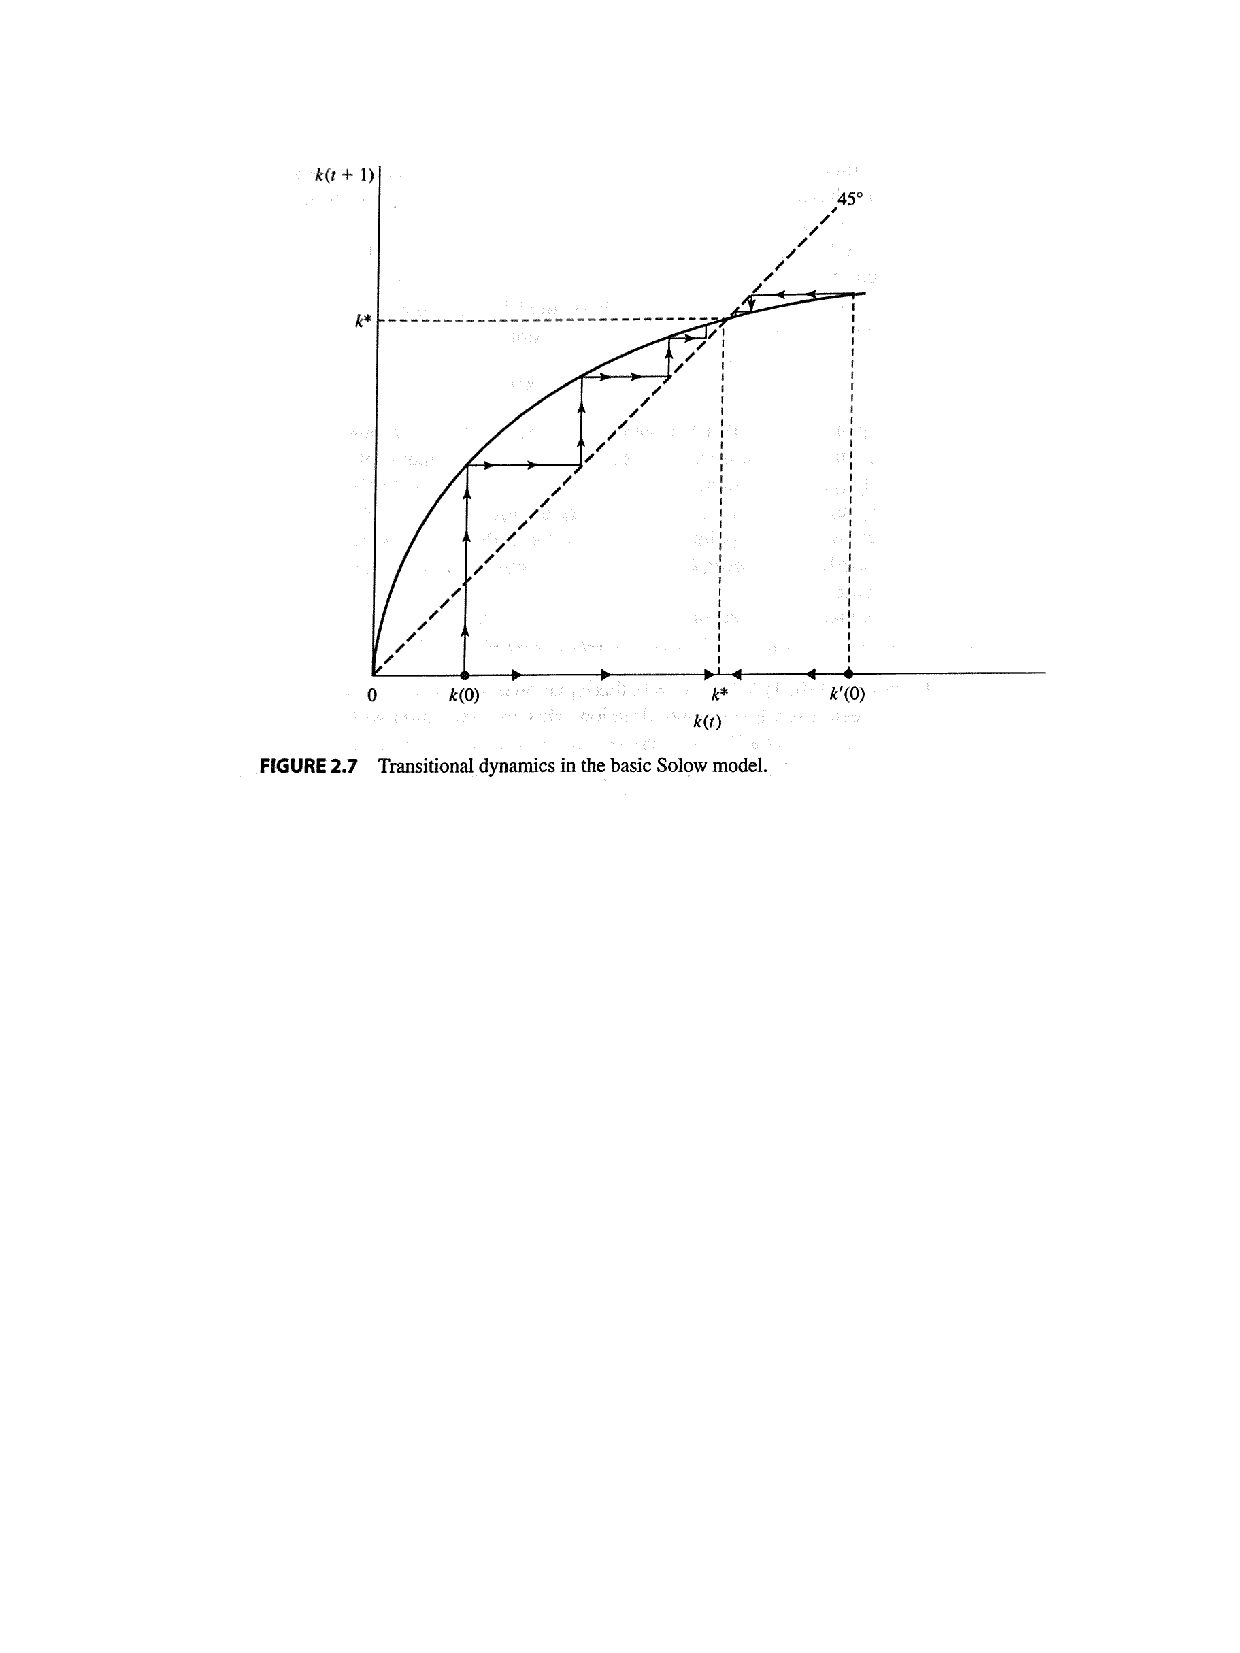
\includegraphics[scale=0.5]{./solow_transition_acemoglu.pdf}
\end{figure}
\end{frame}



%%%%%%%%%%%%%%%%%%%%%%%%%%  SLIDE   %%%%%%%%%%%%%%%%%%%%%%%%%%%%%%%%
\begin{frame}{6. Stochastic Difference Equations}
\begin{itemize}
\item Consider the process $\{X_t\}$ with 
\begin{equation}\label{eq:stochastic_difference}
	X_{t+1} = A X_t + Cw_{t+1}
\end{equation}
where $w_{t+1}$ is an iid. process with $w_{t+1} \sim \mathcal N(0, 1)$

\item Equation \eqref{eq:stochastic_difference} is a \textit{first-order, linear stochastic difference equation}

\item Let $\mathbb E_t$ the \textit{conditional expectation} operator (conditional on time $t$ information)

\item For example:
\begin{align*}
	\mathbb E_t(X_{t+1}) &= \mathbb E(X_{t+1} \mid X_t) = \mathbb E(A X_t + Cw_{t+1} \mid X_t) \\
	&= A X_t + C \mathbb E(w_{t+1} \mid X_t) = A X_t + C \mathbb E(w_{t+1}) = A X_t
\end{align*}
\end{itemize}
\end{frame}


%%%%%%%%%%%%%%%%%%%%%%%%%%  SLIDE   %%%%%%%%%%%%%%%%%%%%%%%%%%%%%%%%
\begin{frame}{}
\begin{itemize}
\item Rational expectations: agents' beliefs about stochastic processes are consistent with the true distribution of the process

\item Consumption Euler equation with uncertainty (e.g., stochastic income):
\begin{equation*}
	u'(C_t) = \beta R \mathbb E_t \Big[ u'(C_{t+1}) \Big]
\end{equation*}

\item New Keynesian Phillips curve with uncertainty (e.g., demand shocks):
\begin{equation*}
	\pi_t = \beta \mathbb E_t \Big[ \pi_{t+1} \Big] + \kappa x_t
\end{equation*}
\end{itemize}
\end{frame}










%%%%%%%%%%%%%%%%%%%%%%%%%%%%%%%%%%%%%%%%%%%%%%%%%%%%%%%%%%%%%%
%%%%%%%%%%%%%%%%%%%%%%%%%%%%%%%%%%%%%%%%%%%%%%%%%%%%%%%%%%%%%%
%%%%%%%%%%%%%%%%%%%%%%%%%%%%%%%%%%%%%%%%%%%%%%%%%%%%%%%%%%%%%%

\appendix


\end{document}









